\documentclass[10pt]{article}


\usepackage{amssymb,amsthm,amsmath}
\usepackage{enumerate}
\usepackage{graphicx,color}
\usepackage[hidelinks]{hyperref}
%\usepackage{refcheck}

\newcommand{\dd}{\mathrm{d}}
\newcommand{\E}{\mathbb{E}}
\newcommand{\1}{\textbf{1}}
\newcommand{\R}{\mathbb{R}}
\newcommand{\C}{\mathbb{C}} 
\newcommand{\Z}{\mathbb{Z}}
\newcommand{\N}{\mathbb{N}}
\newcommand{\scal}[2]{\left\langle #1, #2 \right\rangle}
\newcommand{\red}{\color{red}}
\newcommand{\shift}{\vdash}
\newcommand{\pP}{\mathcal{P}}
\newcommand{\lL}{\mathcal{L}}

\DeclareMathOperator{\Var}{Var}
\DeclareMathOperator{\sgn}{sgn}

\usepackage[paper=a4paper, left=1.3in, right=1.3in, top=1in, bottom=1in]{geometry}
\linespread{1.3}
\pagestyle{plain}

\newtheorem{theorem}{Theorem}
\newtheorem{lemma}[theorem]{Lemma}
\newtheorem{corollary}[theorem]{Corollary}

\theoremstyle{remark}
\newtheorem{remark}[theorem]{Remark}


\newtheorem{conjecture}{Conjecture}

\theoremstyle{definition}
\newtheorem{definition}[theorem]{Definition}

\theoremstyle{prop}
\newtheorem{prop}[theorem]{Prop}

\theoremstyle{Corollary}
\newtheorem{Corollary}[theorem]{Corollary}


\title{\vspace{-3em}Log}



\begin{document}

\section{Lambert Calculation}

Note: These are distributions of characteristics

Note: Variances of these distributions should be the same.

%May be some issues with constants in from of functions, but whatever

$f(x) = e^{-3x^2/2}$(characteristic of gaussian with variance 3)

Set $g(x) = e^{-x^2/2}|1-x^2|$.(norm of characteristic of density $e^{-x^2/2}x^2$)

We seek to compute $\mu\{ x > 0: e^{-x^2/2}|1-x^2| < t\}$ for $0 < t < 1$ where $d\mu = \frac{1}{x^{p+1}} dx$ for $p > 2$

Looking at the graph:

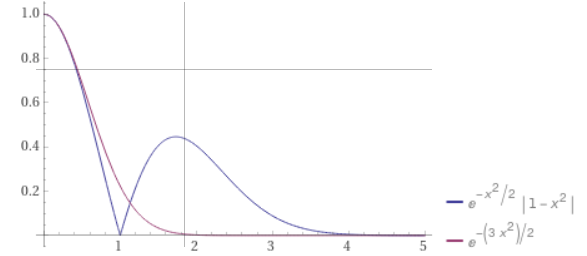
\includegraphics[width=250px]{pictures/ex2absdist.PNG}

Let F be the modified distribution of $e^{-x^2/2}$ and G be the modified distribution of the other. Set $y_{lm}$ to be the local max of f away from 0. Then clearly for $t \geq y_{lm}$, $G(t) \geq F(t)$ since f dominates over $x$ s.t. $g(x) > t_{lm}$. So it suffices to comopute the measure for t in the interval $(0,y_{lm})$. 

We see this is the measure of two intervals: one containing 1 and one from some $(x,\infty)$. Call these $(x_{+,0)},x_{-,0})$ and $(x_{-,-1},\infty)$. We must compute these in terms of the lambert W function.

For $t \in (0,y_{lm})$ write for $x > 0$

\begin{align*}
	e^{-x^2/2}|1-x^2| = t \iff |y|e^y = \frac{e^{1/2}}{2}t
\end{align*}

where $y = \frac{1-x^2}{2}$. We case if $y > 0$. 

If $y \geq 0$ then $0 < x < 1$. In this case we have $ye^y = \frac{e^{1/2}}{2}t$ which we can solve with the lambert $W_0$ function yielding $y = W_0(\frac{e^{1/2}}{2}t)$.

In the case $y < 0$ then $x > 1$ and we have two possible solutions to $|y|e^y = \frac{e^{1/2}}{2}t$. Write $-y e^y = \frac{e^{1/2}}{2}t \implies y \iff y e^y = -\frac{e^{1/2}}{2}t$ which is solved by $y = W_0(-\frac{e^{1/2}}{2}t)$ and $y = W_{-1}(-\frac{e^{1/2}}{2}t)$. 

Label

\begin{align*}
	x_{+,0} = \sqrt{1 - 2W_0(\frac{e^{1/2}}{2}t)}\\
	x_{-,0} = \sqrt{1 - 2W_0(-\frac{e^{1/2}}{2}t)}\\
	x_{-,-1} = \sqrt{1-2W_{-1}(\frac{e^{1/2}}{2}t)}
\end{align*}

Note: $W_{-1}(\frac{e^{1/2}}{2}t) \leq W_{0}(\frac{e^{1/2}}{2}t)$ so $x_{-,0} \leq x_{-,-1}$

Then we can compute 

\begin{align*}
	\mu\{ x > 0: e^{-x^2/2}|1-x^2| < t\} &= \int_{(x_{+,0},x_{-,0})} \frac{1}{x^{p+1}} dx + \int_{(x_{-,-1},\infty)} \frac{1}{x^{p+1}}dx = \\
	& -\frac{1}{p}x^{-p}|_{x_{-,0},x_{+,0}} + (-\frac{1}{p}x^{-p})|_{\infty,x_{-,-1}} = \\
	& -\frac{1}{p}[(1 - 2W_0(-\frac{e^{1/2}}{2}t))^{-p/2} - (1 - 2W_0(\frac{e^{1/2}}{2}t))^{-p/2} - (1 - 2W_{-1}(-\frac{e^{1/2}}{2}t))^{-p/2}]
\end{align*}

Note: This formula valid for $t < t_{lm}$. We can compute $t_{lm} = 2e^{-3/2}$ via calculus.

\end{document}



